% !TEX root = /doc.tex

\section{Evaluation}

\subsection{Evaluation metrics}

The evaluation metrics collected to compare the classifiers come from the field of information retrieval and are considered standard metrics for their purpose \cite{Sammut2017}. Most of these metrics can be calculated using values from a so-called confusion matrix and all of them measure the performance of the predictions of classifiers from different points of view. In the case of a binary classification, as this work was based on, this matrix consists of four groups whose values indicate whether the respective classifier could correctly or incorrectly assign an object to one of the two target classes \cite{Sammut2017}. In connection with such matrices, the two target classes are called "positive" and "negative". For this work the positive class is assigned to the label "defective" and the negative class to the label "clean". The form of a general confusion matrix is shown in \autoref{fig:confu}.

\begin{figure}[H]
    \centering
    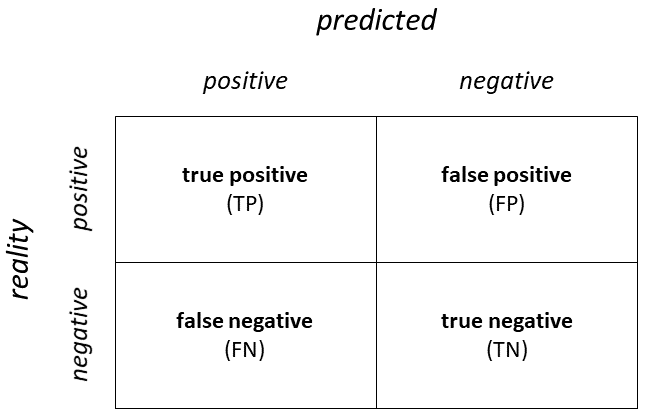
\includegraphics[width=0.4\textwidth]{Confusion}
    \caption{general confusion matrix\label{fig:confu}}
\end{figure}

The WEKA tool used for training the classifiers has the option of outputting confusion matrices for the tests performed on the classifiers. Based on the values of the assignments to the groups mentioned above, the following evaluation metrics were calculated:

\begin{itemize}
\item Accuracy
\\This value measures the accuracy of the classifier's predictions and indicates to what extent its predictions agree with the modelled reality \cite{Sammut2017}. The formula for calculating the accuracy is:
\\\[\text{Accuracy} = \frac{TP+TN}{TP+TN+FP+FN}\]
The result of the calculation is a percentage value. $100\%$ represents the best possible accuracy. In this case, all predictions are correct and correspond to reality.
\item True-Positive-Rate (TP rate) / Recall
\\This value indicates the proportion of correctly positive predictions of all positive predictions \cite{Alpaydin2010}. The formula for calculating the TP rate or recall is
\\\[\text{TP rate} = \frac{TP}{TP+FN}\]
The result of the calculation is a percentage value. $100\%$ thus represents the best possible TP rate or recall. In this case all positive predictions are made correctly. Both terms are used in parallel to calculate the formula shown.
\item Precision
\\ This value indicates the number of positive predictions that actually belong to the positive class \cite{Sammut2017}. The formula for determining the precision is
\\\[\text{Precision} = \frac{TP}{TP+FP}\]
The result of the calculation is a percentage value. $100\%$ represents the best possible precision. In this case only correct positive predictions are made.
\item F score
\\ This value calculates the harmonic mean of the Precision and Recall values and is therefore between these two values, but closer to the smaller value \cite{Sammut2017}. The formula for calculating the F score is
\\\[\text{F score} = \frac{2TP}{2TP+FP+FN}\]
The result of the calculation is a percentage value. $100\%$ represents the best possible F score. In this case, all positive predictions were made correctly.
\end{itemize}

In order to obtain a further measure of the prediction performance and the quality of the predictions, the so-called ROC curves (ROC = Receiver Operating characteristic) of the individual classifiers were determined. These have the advantage that they represent the performance of the classifiers in a simple and understandable way and make the quality of the predictions "visible". For this purpose, it is sufficient to know the standard progression of the curves, which will be illustrated in the following example.
The ROC curves are probability distributions that describe the relationship between the TP rate (y axis) and the false positive rate (x axis) \cite{Sammut2017}. The False-Positive-Rate (FP rate) indicates the proportion of predictions that are incorrectly evaluated as positive \cite{Alpaydin2010}. It is calculated using the following formula:
\\\[\text{FP rate} = \frac{FP}{FP+TN}\]
As with all metrics, the result of the FP rate is a percentage value. In contrast to the previous metrics, this result should at best be as low as possible. Both the TP rate and the FP rate give only singular values, from which no graphs can be derived. However, when predicting a data point, each classifier calculates probabilities that represent the affiliation to the values of the target class. As a rule, a data point is assigned to the positive class if the probability exceeds a threshold value of $0.5$ - data points that fall below this threshold value are assigned to the negative class. If the threshold value is increased, fewer data points are assigned to the positive class, whereas if the threshold value is lowered, more data points are assigned to the positive class. For the creation of the ROC curves, the values of the TP rate and FP rate are thus compared, taking into account the threshold values in the range of $0.0$ to $1.0$.
Another metric that occurs in conjunction with the ROC curve is the ROC area. This value, which is calculated using the ROC curve and is also called AUC area (AUC = Area Under Curve), indicates the extent to which a classifier is able to distinguish between the values of the target classes. The higher this value is ($1.0$ is the maximum), the better the classifier can make correct predictions. It therefore reflects the quality of the predictions.
All presented metrics are automatically calculated by WEKA. The tool also has the ability to output ROC curves with the corresponding ROC areas. The values of the metrics determined during the evaluation of the classifiers as well as the ROC curves and areas of the ROC ranges are listed, compared and interpreted in the following section.

\subsection{Results}

Lorem ipsum.

\subsubsection*{Results and comparison of the feature-based classifiers}

Lorem ipsum.

\subsubsection*{Results and comparison of the file-based classifiers}

Lorem ipsum.